\documentclass{article}

\usepackage{Zelig}



\usepackage{Sweave}
\begin{document}
\nobibliography*


\section{{\tt poisson}: Poisson Regression for Event Count
Dependent Variables}\label{poisson}

Use the Poisson regression model if the observations of your dependent
variable represents the number of independent events that occur during
a fixed period of time (see the negative binomial model, \Sref{negbin},
for over-dispersed event counts.)  For a Bayesian implementation of
this model, see \Sref{poisson.bayes}.  

\subsubsection{Syntax}

\begin{verbatim}
> z.out <- zelig(Y ~ X1 + X2, model = "poisson", data = mydata)
> x.out <- setx(z.out)
> s.out <- sim(z.out, x = x.out)
\end{verbatim}

\subsubsection{Additional Inputs} 

In addition to the standard inputs, {\tt zelig()} takes the following
additional options for poisson regression:  
\begin{itemize}
\item {\tt robust}: defaults to {\tt FALSE}.  If {\tt TRUE} is
selected, {\tt zelig()} computes robust standard errors via the {\tt
sandwich} package (see \cite{Zeileis04}).  The default type of robust
standard error is heteroskedastic and autocorrelation consistent (HAC),
and assumes that observations are ordered by time index.

In addition, {\tt robust} may be a list with the following options:  
\begin{itemize}
\item {\tt method}:  Choose from 
\begin{itemize}
\item {\tt "vcovHAC"}: (default if {\tt robust = TRUE}) HAC standard
errors. 
\item {\tt "kernHAC"}: HAC standard errors using the
weights given in \cite{Andrews91}. 
\item {\tt "weave"}: HAC standard errors using the
weights given in \cite{LumHea99}.  
\end{itemize}  
\item {\tt order.by}: defaults to {\tt NULL} (the observations are
chronologically ordered as in the original data).  Optionally, you may
specify a vector of weights (either as {\tt order.by = z}, where {\tt
z} exists outside the data frame; or as {\tt order.by = \~{}z}, where
{\tt z} is a variable in the data frame).  The observations are
chronologically ordered by the size of {\tt z}.
\item {\tt \dots}:  additional options passed to the functions 
specified in {\tt method}.   See the {\tt sandwich} library and
\cite{Zeileis04} for more options.   
\end{itemize}
\end{itemize}

\subsubsection{Example}

Load sample data:  
\begin{Schunk}
\begin{Sinput}
> data(sanction)
\end{Sinput}
\end{Schunk}
Estimate Poisson model:  
\begin{Schunk}
\begin{Sinput}
> z.out <- zelig(num ~ target + coop, model = "poisson", data = sanction)
\end{Sinput}
\end{Schunk}
\begin{Schunk}
\begin{Sinput}
> summary(z.out)
\end{Sinput}
\end{Schunk}
Set values for the explanatory variables to their default mean values:  
\begin{Schunk}
\begin{Sinput}
> x.out <- setx(z.out)
\end{Sinput}
\end{Schunk}
Simulate fitted values:  
\begin{Schunk}
\begin{Sinput}
> s.out <- sim(z.out, x = x.out)
\end{Sinput}
\end{Schunk}
\begin{Schunk}
\begin{Sinput}
> summary(s.out)
\end{Sinput}
\end{Schunk}
\begin{center}
\begin{Schunk}
\begin{Sinput}
> plot(s.out)
\end{Sinput}
\end{Schunk}
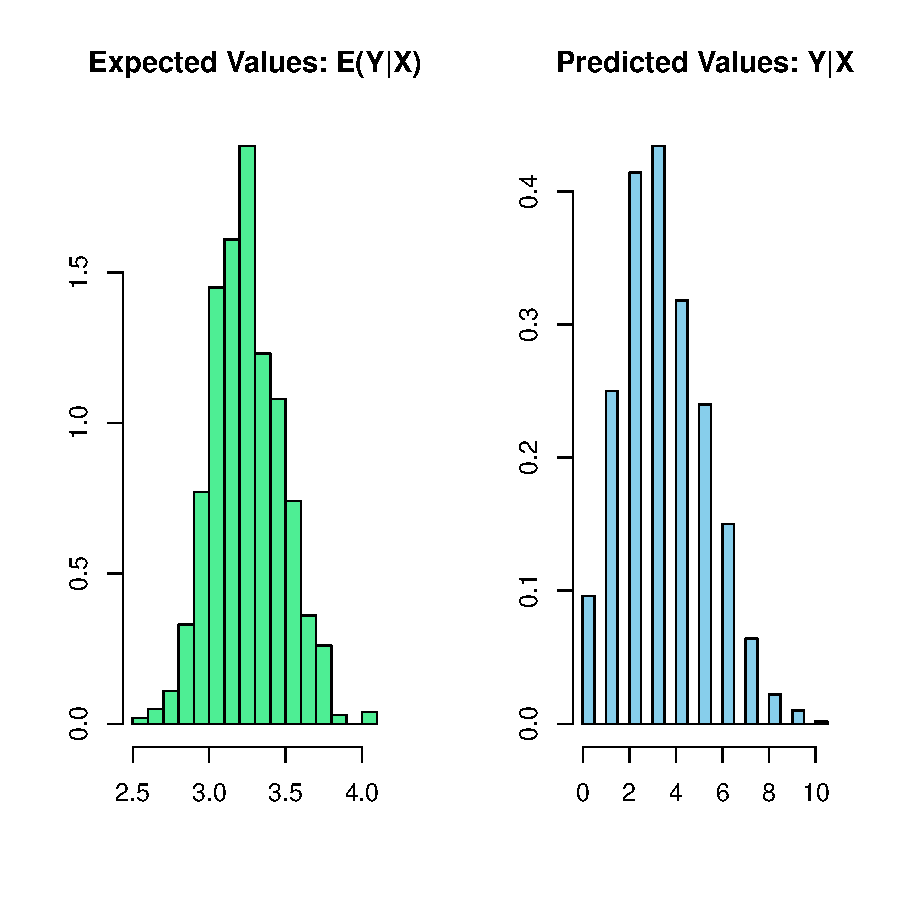
\includegraphics{vigpics/poisson-ExamplePlot}
\end{center}

\subsubsection{Model}
Let $Y_i$ be the number of independent events that occur during a
fixed time period. This variable can take any non-negative integer.

\begin{itemize}
\item The Poisson distribution has \emph{stochastic component}
  \begin{equation*}
    Y_i \; \sim \; \textrm{Poisson}(\lambda_i),
  \end{equation*}
  where $\lambda_i$ is the mean and variance parameter.
  
\item The \emph{systematic component} is 
  \begin{equation*}
    \lambda_i \; = \; \exp(x_i \beta),
  \end{equation*}
  where $x_i$ is the vector of explanatory variables, and $\beta$ is
  the vector of coefficients.
\end{itemize}

\subsubsection{Quantities of Interest}

\begin{itemize}
  
\item The expected value ({\tt qi\$ev}) is the mean of simulations
  from the stochastic component, $$E(Y) = \lambda_i =  \exp(x_i
  \beta),$$ given draws of $\beta$ from its sampling distribution.  
  
\item The predicted value ({\tt qi\$pr}) is a random draw from the
  poisson distribution defined by mean $\lambda_i$.

\item The first difference in the expected values ({\tt qi\$fd}) is given by:
\begin{equation*}
\textrm{FD} \; = \; E(Y | x_1) - E(Y \mid x)
\end{equation*}
\item In conditional prediction models, the average expected treatment
  effect ({\tt att.ev}) for the treatment group is 
    \begin{equation*} \frac{1}{\sum_{i=1}^n t_i}\sum_{i:t_i=1}^n \left\{ Y_i(t_i=1) -
      E[Y_i(t_i=0)] \right\},
    \end{equation*} 
    where $t_i$ is a binary explanatory variable defining the treatment
    ($t_i=1$) and control ($t_i=0$) groups.  Variation in the
    simulations are due to uncertainty in simulating $E[Y_i(t_i=0)]$,
    the counterfactual expected value of $Y_i$ for observations in the
    treatment group, under the assumption that everything stays the
    same except that the treatment indicator is switched to $t_i=0$.

\item In conditional prediction models, the average predicted treatment
  effect ({\tt att.pr}) for the treatment group is 
    \begin{equation*} \frac{1}{\sum_{i=1}^n t_i}\sum_{i:t_i=1}^n \left\{ Y_i(t_i=1) -
      \widehat{Y_i(t_i=0)} \right\},
    \end{equation*} 
    where $t_i$ is a binary explanatory variable defining the
    treatment ($t_i=1$) and control ($t_i=0$) groups.  Variation in
    the simulations are due to uncertainty in simulating
    $\widehat{Y_i(t_i=0)}$, the counterfactual predicted value of
    $Y_i$ for observations in the treatment group, under the
    assumption that everything stays the same except that the
    treatment indicator is switched to $t_i=0$.
\end{itemize}

\subsubsection{Output Values}

The output of each Zelig command contains useful information which you
may view.  For example, if you run \texttt{z.out <- zelig(y \~\,
  x, model = "poisson", data)}, then you may examine the available
information in \texttt{z.out} by using \texttt{names(z.out)},
see the {\tt coefficients} by using {\tt z.out\$coefficients}, and
a default summary of information through \texttt{summary(z.out)}.
Other elements available through the {\tt \$} operator are listed
below.

\begin{itemize}
\item From the {\tt zelig()} output object {\tt z.out}, you may extract:
   \begin{itemize}
   \item {\tt coefficients}: parameter estimates for the explanatory
     variables.
   \item {\tt residuals}: the working residuals in the final iteration
     of the IWLS fit.
   \item {\tt fitted.values}: a vector of the fitted values for the systemic
     component $\lambda$.  
   \item {\tt linear.predictors}: a vector of $x_{i}\beta$.  
   \item {\tt aic}: Akaike's Information Criterion (minus twice the
     maximized log-likelihood plus twice the number of coefficients).
   \item {\tt df.residual}: the residual degrees of freedom.
   \item {\tt df.null}: the residual degrees of freedom for the null
     model.
   \item {\tt zelig.data}: the input data frame if {\tt save.data = TRUE}.  
   \end{itemize}

\item From {\tt summary(z.out)}, you may extract: 
   \begin{itemize}
   \item {\tt coefficients}: the parameter estimates with their
     associated standard errors, $p$-values, and $t$-statistics.
   \item{\tt cov.scaled}: a $k \times k$ matrix of scaled covariances.
   \item{\tt cov.unscaled}: a $k \times k$ matrix of unscaled
     covariances.  
   \end{itemize}

\item From the {\tt sim()} output object {\tt s.out}, you may extract
  quantities of interest arranged as matrices indexed by simulation
  $\times$ {\tt x}-observation (for more than one {\tt x}-observation).
  Available quantities are:

   \begin{itemize}
   \item {\tt qi\$ev}: the simulated expected values given the
     specified values of {\tt x}.
   \item {\tt qi\$pr}: the simulated predicted values drawn from the
     distributions defined by $\lambda_i$.
   \item {\tt qi\$fd}: the simulated first differences in the expected
     values given the specified values of {\tt x} and {\tt x1}.
   \item {\tt qi\$att.ev}: the simulated average expected treatment
     effect for the treated from conditional prediction models.  
   \item {\tt qi\$att.pr}: the simulated average predicted treatment
     effect for the treated from conditional prediction models.  
   \end{itemize}
\end{itemize}

\subsection* {How to Cite} 

How to cite this model in Zelig:
\begin{verse}
  Kosuke Imai, Gary King, and Olivia Lau. 2007. "poisson: Poisson Regression for Event Count Dependent Variables" in Kosuke Imai, Gary King, and Olivia Lau, "Zelig: Everyone's Statistical Software,"http://gking.harvard.edu/zelig
\end{verse}
\CiteZelig
\subsection* {See also}
The poisson model is part of the stats package by \citet{VenRip02}.
Advanced users may wish to refer to \texttt{help(glm)} and
\texttt{help(family)}, as well as \cite{McCNel89}. Robust standard
errors are implemented via the sandwich package by \citet{Zeileis04}.
Sample data are from \cite{Martin92}.

\bibliographystyle{asa}
\bibliography{gk,gkpubs}
 \end{document}


%%% Local Variables: 
%%% mode: latex
%%% TeX-master: t
%%% End: 
